%%%%%%%%%%%%%%%%%%%%%%%%%%%%%%%%%%%%%%%%%%%%%%%%%%%%%%
%%%%%%%%%%%%%%%%%%%%%%%%%%%%%%%%%%%%%%%%%%%%%%%%%%%%%%%%%%%%%%%%%%%%
\def\scl{1}%scaling factor of the picture


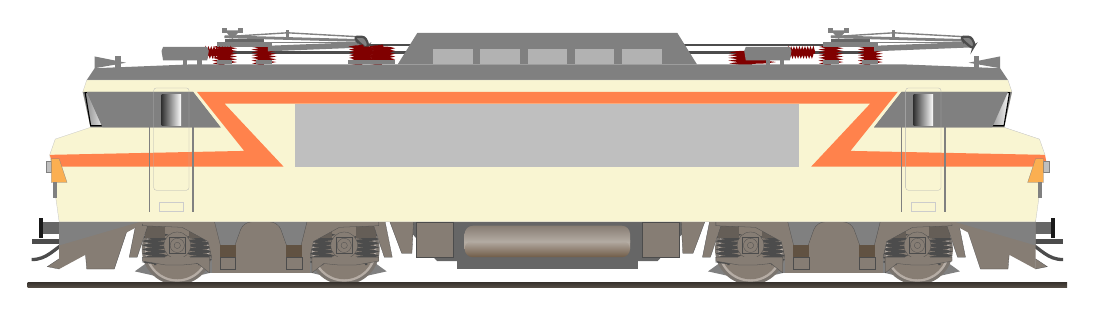
\begin{tikzpicture}[
  scale=\scl,
  beige/.style={color=gray!20!brown!40!yellow!20!},
  orange/.style={color=red!70!yellow!70!},
  wagon/.style={green!70!brown!20!black!75!,draw=black,thick},
  fenetre/.style={white,rounded corners = 2pt,draw=black, thick},
  porte/.style={red!55!black,draw=gray!20!, ultra thin},
  porteMotrice/.style={rounded corners = 1pt,draw=gray!60!, ultra thin},
  essieux/.style={gray!20!brown!30!black!60!,draw=black!70!, ultra thin},
  grisEssieux/.style={gray!20!brown!30!black!60!}
]

  \begin{scope}[xshift=0 cm,yshift=0 cm]%, scale = 0.3
%
%         LIAISONS
%
 \draw[black!70!, very thick] % liaison souple
    (6.1,0.65) to[out=330,in=180] (6.55,0.42);
 \draw[black!70!, very thick] 
    (-6.1,0.65) to[out=210,in=0] (-6.55,0.42);

  \foreach \t in {-1, 1}
  {
    \coordinate (A) at (6.1 * \t,0.65) ;
    \coordinate (B) at (6.55 * \t,0.65) ;
 \draw[black!70!, ultra thick] 
    (A) -- (B);

  }

 % BUTOIRS
 %(\t * 6.1, 0.75) rectangle (\t * 6.4, 0.9);
 %(\t * 6.4, 0.7) rectangle (\t * 6.45, 0.95);

 % ESSIEUX derrière les roues

  \foreach \x in {3.64, -3.64}
   {
 \fill[gray] 
  (\x - 0.65, 0.95) -- (\x + 0.65, 0.95) --
 (\x + 1.6, 0.27) -- (\x + 1.06, 0.15) -- (\x + 0.65, 0.25)
 -- (\x - 0.65, 0.25) -- (\x - 1.06, 0.15) -- (\x - 1.6, 0.27) -- cycle;
  }

%  ROUES

\def\hauteur{0.55}% de l'axe des roues
\foreach \x in {2.58, 4.7, -4.7, -2.58}
  {
 % gris essieux : gray!20!brown!30!black!50!
    \fill[gray!20!brown!20!black!60!] (\x, \hauteur) circle (0.45 cm);
    \fill[gray!20!brown!40!black!40!] (\x, \hauteur) circle (0.41 cm);
    \fill[gray!10!brown!30!black!60!] (\x, \hauteur) circle (0.38 cm);

% RESSORT

  \foreach \t in {-1,1}
  {
     \draw[decorate, decoration={snake, segment length=1.5pt, amplitude=1.2mm}, black!70!, thick]
       (\x + \t * 0.28, 0.75) -- (\x + \t * 0.28, 0.35);
    % RESSORT fixation supérieur
     \fill[gray!20!brown!20!black!70!]
       (\x + \t * 0.28 - .13, 0.9) rectangle (\x + \t * 0.28 + .13, 0.7);
  }
  }


 % ESSIEUX devant les roues

\def\y{0.2}
  \foreach \x in {3.64, -3.64}
{
  \foreach \t in {-1,1}
  {
  % détail
 \fill[essieux] (\x + \t*1.57, 0.95) -- (\x + \t*1.67, 0.45) --
 (\x + \t*1.57, 0.45) -- (\x + \t*1.4, 0.95) -- cycle;

  %  montants supérieur
 \fill[essieux] (\x + \t*1.5, 0.95) -- (\x + \t*1.5, 0.85) -- (\x + \t*1, 0.83) -- (\x + \t*0.67, 0.65)
 -- (\x + \t*0.6, 0.35) -- (\x + \t*0.45, 0.35) -- (\x + \t*0.6, 0.95) -- cycle;


    %  montant inférieur
 \fill[essieux] (\x + \t * 1.5,0.45) -- (\x + \t * 1.5,0.4) -- (\x + \t * 1.2,0.35) -- (\x + \t * 1,0.35)
 -- (\x + \t * 0.80,0.37) -- (\x + \t * 0.65,0.25) -- (\x + \t * 0.65,0.45) -- cycle;

 \fill[essieux] (\x + \t*1.06, \hauteur + 0.05) circle (0.17 cm);
 \fill[grisEssieux]
 (\x + \t*1.06 + 0.16, 0.45) rectangle (\x + \t*1.06 + -0.16, 0.37);
 \fill[essieux]
 (\x + \t*1.06 + 0.1, \hauteur + 0.05 + -0.1) rectangle (\x + \t*1.06 + -0.1, \hauteur + 0.05 + 0.1);
    \fill[essieux] (\x + \t*1.06, \hauteur + 0.05) circle (0.09 cm);
    \fill[essieux] (\x + \t*1.06, \hauteur + 0.05) circle (0.04 cm);

  }

    %  milieux
   \fill[essieux, rounded corners = 3pt]
  (\x-0.22, 0.9) -- (\x + 0.22, 0.9) -- (\x + 0.4, 0.4) -- (\x - 0.4, 0.4) -- cycle;

    %  milieux inférieur 
  \fill[grisEssieux]
  (\x - 0.62,0.5) -- (\x + 0.62,0.5) -- (\x + 0.62,0.25) -- (\x - 0.62,0.25) -- cycle;

  \foreach \t in {-1,1}    % silent bloc
  {
  \fill[brown!30!black!80!]
 (\x + \t * 0.42 - 0.1, 0.6) rectangle (\x + \t * 0.42 + 0.1, 0.4);
  \fill[essieux]
 (\x + \t * 0.42 - 0.1, 0.45) rectangle (\x + \t * 0.42 + 0.1, 0.3);
  }
}

 % DESSOUS

 \fill[black!60!] 
  (1.9, 0.95) -- (- 1.9, 0.95) -- (- 1.4, 0.40) -- (1.4, 0.40) -- cycle;

  \shade[bottom color=gray!10!brown!50!black!60!, top color=gray!20!brown!40!black!40!] % ombre centre cylindre
  (1.05, 0.45) rectangle (-1.05, 0.66);
  \shade[bottom color=gray!20!brown!40!black!40!, top color=gray!10!brown!30!black!60!]
  (1.05, 0.64) rectangle (-1.05, 0.85);

 \fill[black!60!] 
  (2, 0.9) -- (- 2, 0.9) -- (- 1.9, 0.75) -- (1.9, 0.75) -- cycle;
 \fill[black!60!] 
  (1.15, 0.55) -- (- 1.15, 0.55) -- (- 1.15, 0.3) -- (1.15, 0.3) -- cycle;


  \shade[bottom color=brown!40!black!80!, top color=gray!20!brown!40!black!40!, rounded corners = 3pt]% cylindre
  (1.05, 0.45) rectangle (-1.05, 0.66);
  \shade[bottom color=gray!20!brown!40!black!40!, top color=gray!10!brown!30!black!60!, rounded corners = 3pt]%, shading angle={90}
  (1.05, 0.64) rectangle (-1.05, 0.85);

  \foreach \t in {-1,1}
{
  \fill[essieux] % details 1
 (\t * 2, 0.9) -- (\t * 1.7, 0.9) -- (\t * 1.72, 0.5)
 -- (\t * 1.85, 0.5) --  cycle;
  \fill[essieux] % details 2
 (\t * 1.67, 0.9) -- (\t * 1.2, 0.9) -- (\t * 1.2, 0.45)
 -- (\t * 1.67, 0.45) --  cycle;
}

 % BUTOIRS
\foreach \t in {-1,1}
{
  \fill[color=gray!80!black] % 
 (\t * 6.1, 0.75) rectangle (\t * 6.4, 0.9);
  \fill[color=black!80!gray] % plaques
 (\t * 6.4, 0.7) rectangle (\t * 6.45, 0.95);
}

% BAS DE CAISSE

\foreach \t in {-1,1}
{

  \fill[essieux] % details
 (\t * 5.9, 0.9) -- (\t * 5.3, 0.9) -- (\t * 5.5, 0.3)
 -- (\t * 5.85, 0.3) --  cycle;

  \fill[essieux] % pare bufle
 (\t * 6.2, 0.43) -- (\t * 6.35, 0.33) -- (\t * 6.2, 0.3) --  cycle;
  \fill[grisEssieux] % pare bufle
 (\t * 5, 0.95) -- (\t * 6.2, 0.95) -- (\t * 6.2, 0.3) --  cycle;

  \fill[color=gray] % carrosserie
 (\t * 5, 0.95) -- (\t * 6.2, 0.95) -- (\t * 6.2, 0.6) --  cycle;
}


%
%     CORPS DE LA MOTRICE
%
% liaisons électriques entre caténaires
     \draw[black!70!, thick] (-2.4, 3.15) -- (3.9, 3.15);

     \draw[black!70!, thick] (-4.5, 3.05) -- (4.1, 3.05);


%isolant 1
  \foreach \x in {-4.1, -3.6, 3.6, 4.1}
     \draw[decorate, decoration={snake, segment length=1pt, amplitude=0.8mm}, red!50!black, thick]
       (\x, 2.9) -- (\x, 3.15);
  \foreach \x in {-4.1, -3.6, 3.6, 4.1}
     \fill[gray]
       (\x - 0.1, 2.9) rectangle (\x + 0.1, 2.95);

%caténaire
\def\h{0.05}
  \foreach \x in {-4.1, 3.6}
  {
     \draw[gray, line width=2pt] (\x + 0.6, 3.1+\h) -- (\x - 0.1, 3.1+\h);
     \draw[black!60!, line width=1pt] (\x + 0.5, 3.15+\h) -- (\x, 3.15+\h);

     \draw[gray, line width=2pt] (\x + 0.55, 3.05+\h) -- (\x + 1.8, 3.1+\h);
     \draw[gray, line width=.5pt] (\x + 0.55, 3.13+\h) -- (\x  + 1.8, 3.13+\h);

     \draw[gray, line width=1pt] (\x, 3.2+\h) -- (\x  + 1.8, 3.15+\h);
     \draw[gray, line width=.5pt] (\x, 3.2+\h) -- (\x  + .8, 3.25+\h) -- (\x  + 1.7, 3.2+\h);
     \draw[gray, line width=1pt] (\x  + .8, 3.18+\h) -- (\x  + .8, 3.28+\h);

  \fill[gray, draw=black!70!, thick, rounded corners = 1pt]% coude
 (\x + 1.8, 3.05+\h) -- (\x + 1.83, 3.1+\h) -- (\x + 1.78, 3.2+\h) -- (\x + 1.65, 3.2+\h)
 -- (\x + 1.68, 3.15+\h) -- cycle;

  }
  \foreach \x in {-4, 3.7}
  {
  \fill[gray, line width=2pt]% support et capteurs
 (\x-0.1, 3.28+\h) -- (\x+0.1, 3.28+\h) -- (\x, 3.17+\h)  -- cycle;
     \draw[gray, line width=2pt] (\x-0.07, 3.28+\h) -- (\x-0.13, 3.28+\h);
     \draw[gray, line width=2pt] (\x+0.07, 3.28+\h) -- (\x+0.13, 3.28+\h);
  }

% ÉLÉMENTS CATÉNAIRES

%isolant 2 à gauche
  \foreach \x in {-2.1, -2.35}
     \draw[decorate, decoration={snake, segment length=1pt, amplitude=1.1mm}, red!50!black, thick]
       (\x, 2.9) -- (\x, 3.15);
     \fill[gray] (-2.23 - 0.3, 2.9) rectangle (-2.23 + 0.3, 2.95);
     \fill[gray] (-2.23 - 0.3, 2.9) rectangle (-2.23 + 0.3, 2.95);
%isolant 2 à droite
     \draw[decorate, decoration={snake, segment length=1pt, amplitude=2mm}, red!50!black, thick]
       (2.6, 2.9) -- (2.6, 3.08);
   %  \fill[gray] (2.6 - 0.3, 2.9) rectangle (2.6 + 0.3, 2.95);
% boitier
  \foreach \x in {-4.6, 2.8}
{
     \draw[decorate, decoration={snake, segment length=1pt, amplitude=0.4mm}, red!50!black, thick]
       (\x+0.25, 3.05) -- (\x+0.6, 3.05);

     \fill[gray] (\x - 0.28, 3.12) -- (\x + 0.28, 3.12)
     -- (\x + 0.3, 3.07)
     -- (\x + 0.28, 2.95) -- (\x - 0.28, 2.95) -- (\x - 0.3, 3.07) -- cycle;

     \draw[gray, ultra thick] (\x + 0.18, 3.12) -- (\x + 0.18, 2.5);
     \draw[gray, ultra thick] (\x, 3.12) -- (\x, 2.5);
}


% trompes
\foreach \t in {-1, 1}
  {
  \fill[gray]%
 (\t * 5.35,2.92) -- (\t * 5.75, 3) -- (\t * 5.75, 2.85)  -- cycle;
  \draw[gray, line width=2pt] (\t * 5.45, 3) -- (\t * 5.45, 2.85);
  }


% TOIT

  \fill[color=black!50!] % toit 1
 (1.9, 2.9) -- (-1.9, 2.9) -- (-1.65, 3.3) -- (1.65, 3.3) -- cycle;
\def\demi{0.25}
\foreach \x in{ -1.2, -0.6, 0, 0.6, 1.2 }
  \fill[black!30!] % grilles
 (\x - \demi, 3.1) rectangle (\x + \demi, 2.9);

  \fill[color=gray] % toit 2
 (4.5, 2.9) -- (5.75, 2.85) -- (5.85, 2.7) -- (-5.85, 2.7) -- 
 (-5.75, 2.85) -- (-4.5, 2.9) -- cycle;

  \fill[beige,draw=gray!50!, ultra thin] % carosserie
 (5.85, 2.7) -- (5.9, 2.55) -- (5.8, 2.1) -- (6.25, 1.95) -- (6.32, 1.75)
 -- (6.2, 0.9) --  (-6.2, 0.9) -- (-6.32, 1.75) -- (-6.25, 1.95)
 -- (-5.8, 2.1) -- (-5.9, 2.55) -- (-5.85, 2.7) -- cycle;

  \fill[orange] % décoration
 (4.45, 2.55) -- (3.85, 1.8) -- (6.32, 1.75) -- (6.35, 1.6) -- (3.35, 1.6) -- (4.1, 2.4) 
 -- (-4.1, 2.4) -- (-3.35, 1.6) -- (-6.27, 1.6) -- (-6.32, 1.75) -- (-3.85, 1.8) -- (-4.45, 2.55) -- cycle;


  \fill[color=gray!50!] % grille
 (3.2,1.6) -- (3.2, 2.4) -- (-3.2,2.4) -- (-3.2, 1.6) --  cycle;

  %  FEUX

\foreach \t in {-1,1}
{
  \fill[color=gray!50!,draw=gray, ultra thin]
 (\t * 6.3,1.67) rectangle (\t * 6.37, 1.53);
  \fill[color=brown!20!red!50!yellow!70!,draw=gray, ultra thin]
 (\t * 6.2,1.7) -- (\t * 6.3, 1.7) -- (\t * 6.3, 1.4) -- (\t * 6.1, 1.4) -- cycle;
  \fill[color=gray]
 (\t * 6.23,1.4) rectangle (\t * 6.28, 1.2);
}


\foreach \t in {-1,1}
{
      % PARE BRISE ET GRIS AUTOUR

  \fill[color=gray] % gris
 (\t*4.5, 2.55) -- (\t*5.9, 2.55) -- (\t*5.8, 2.1) -- (\t*4.15, 2.1) --  cycle;
  \shade[bottom color=gray!5!, top color=gray!90!, shading angle={90}, draw=black] % vitre
 (\t*5.8, 2.54) -- (\t*5.87, 2.54) -- (\t*5.8, 2.12) -- (\t*5.6, 2.12) --  cycle;

  \fill[color=gray] % gris
 (\t*4.5, 2.55) -- (\t*5.85, 2.55) -- (\t*5.65, 2.1) -- (\t*4.15, 2.1) --  cycle;

      % PORTES

    \draw[porteMotrice]
 (\t*4.55, 1.3) rectangle (\t*5, 2.6);

    \draw[draw=gray!40!,very thin] % marches
 (\t*4.62, 1.03) rectangle (\t*4.93, 1.15);

    \draw[color=gray] (\t*4.5, 1.03) -- (\t*4.5, 2.3); % rampes
    \draw[color=gray] (\t*5.05, 1.03) -- (\t*5.05, 2.3);

  \shade[bottom color=white, top color=black!80!, shading angle={90}]
   (\t*4.65, 2.12) rectangle (\t*4.9, 2.52); % vitres
}

  % RAIL

  \shade[bottom color=brown!20!gray!60!black, top color=brown!20!gray!40!black]
 (6.6, 0.13) rectangle (-6.6, 0.07);

  \end{scope}
%
%
\end{tikzpicture}
%
